% !TeX encoding = UTF-8
% !TeX spellcheck = en_US
% !TeX root = report1.tex

\section{Variational}
%Now we focus on using the integration to solve the problem established in the introduction.
In this section, we will use the Monte Carlo integration to solve three different problems, the one-dimensional harmonic oscillator, hydrogen atom and helium atom.

\subsection{Harmonic Oscillator}
The Hamiltonian of the harmonic oscillator is
\begin{align*}
	\hat{H} = \frac{-1}{2}\frac{\partial^2}{ \partial x^2} + \frac{1}{2} x^2  \text{~.}
\end{align*}
Where we choose the trial wave function as
\begin{align*}
	\Psi_T = e^{-\alpha x^2} \text{~.}
\end{align*}
With this and eq.~\eqref{eq:local_energy}, we can calculate the local energy:
\begin{align*}
	E_L = \alpha + x^2 \left(\frac{1}{2} - 2\alpha^2\right) \text{~.}
\end{align*}
 	
Notice that, based on the local energy we can already determine that $\alpha = \nicefrac{1}{2}$ gives us the ground state ($E_L = E_0 = \nicefrac{1}{2}$), because in that case the variance of the local energy is equal to zero. It is nonetheless a good test for our algorithm to see if we can find the expected value of $E_0 = \nicefrac{1}{2}$ using Monte Carlo integration.\\
  
We apply the stratified adaptive integration scheme as defined in section~\ref{ch:monte_app} and use Newton's method on the derivative $\frac{dE}{d\alpha} = 2 (\left< E_L \frac{d \ln(\Psi_T)}{d \alpha} \right> - E\left<\frac{d \ln(\Psi_T)}{d \alpha}\right>)$. This method works because our the exact solution is within the family of trial functions, see \cite{JosBook}. %TODO
The new variational parameter can then be adapted as $$\alpha_{\text{new}} = \alpha_{\text{old}} - \gamma \frac{dE}{d\alpha} \text{~.} $$

Two simulations for the one-dimensional harmonic oscillator were performed with 50 iterations, a damping factor of $\gamma = 10^{-5}$, an initial value of $\alpha_i = 3~/~ 0.01$ for alpha and 1,000 test points over a domain with length 4, subdivided into 20 sub-domains for the adaptive grid. With this, we obtained an energy of $E_{MC}-E_0 \simeq 1.63\cdot 10^{-9}$ at $\alpha - \alpha_0 \simeq 7.6455\cdot 10^{-6}$, compare to figure~\ref{fig:Ho_it} and \ref{fig:Ho_rel}.

\begin{figure}[th]
	\begin{center}
		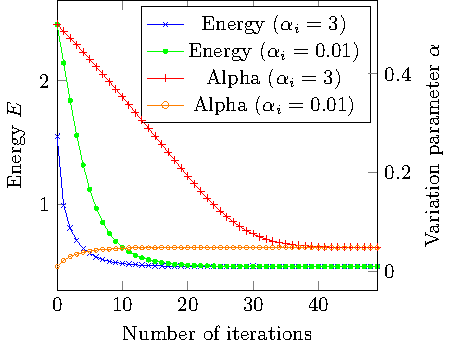
\includegraphics[scale=0.9]{graphs/ho-e-alpha-iterations.pdf}
		\caption{
			Energy and alpha as a function of iteration number. %TODO
			%Calculated $E$ as a function of $\alpha$ using two different starting values for$\alpha_0$. Notice that $\alpha$ converges monotonically (increasing or decreasing) while this is not necessarily true for the energy due to the integration not being exact. Nonetheless, a very accurate result can be found: $E_{\alpha_0 = 0.5} =  $ and $E_{\alpha_0 = 0.5} =  $.
			}
		\label{fig:Ho_it}
	\end{center}
\end{figure}
\begin{figure}[th]
	\begin{center}
		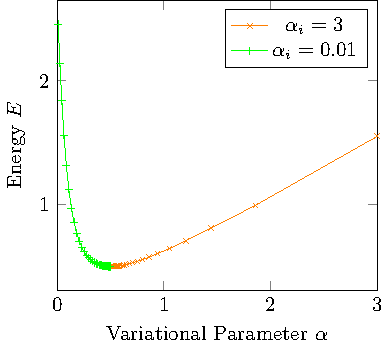
\includegraphics[scale=0.9]{graphs/ho-e-alpha.pdf}
		\caption{
			Energy plotted as a function of alpha. %TODO
			%Calculated $E$ as a function of $\alpha$ using two different starting values for$\alpha_0$. Notice that $\alpha$ converges monotonically (increasing or decreasing) while this is not necessarily true for the energy due to the integration not being exact. Nonetheless, a very accurate result can be found: $E_{\alpha_0 = 0.5} =  $ and $E_{\alpha_0 = 0.5} =  $.
		}
		\label{fig:Ho_rel}
	\end{center}
\end{figure}
  

\subsection{Hydrogen Atom}
We will now consider the Hydrogen atom, where the Hamiltonian is
\begin{align}
  \hat{H} = -\frac{1}{2}\nabla^2 - \frac{1}{r} \text{~.}
\end{align}

We choose the trial wave function as
  \begin{align}
    \Psi_T = e^{-\alpha r} \text{~,}
  \end{align}
which leads to the local energy
  \begin{align}
    E_L(r) = - \frac{1}{r} - \frac{1}{2}\alpha \left(\alpha - \frac{2}{r}\right) \text{~.}
  \end{align}

Here, too, we notice that from inspection it is clear that $\alpha = 1$ yields the ground state energy of $E_L = E_0 = -\nicefrac{1}{2}$, because there $\text{Var}(E_L) = 0$. The convergence on this seems to be quite fast. Using the parameters $\gamma = 5\cdot 10^{-4}$, $\alpha_i = 3 \text{~/~}0.01$ with 5,000 test points over $7$ boxes, we need about 160 iterations to reach $\alpha-\alpha_0 \simeq 5 \cdot 10^{-10}$. That is, within 160 iterations we can estimate $\alpha$ up to ten digits and find the appropriate energy for it. 


\subsection{Helium Atom}
Finally we consider the Hamiltonian for the Helium atom,
\begin{align}
  \hat{H} = -\frac{1}{2} \left(\nabla_{r_1}^2 + \nabla_{r_3}^2 + 2\nabla_{r_1}\cdot \nabla_{r_2}\right)  - \frac{1}{r} \text{~.}
\end{align}
Where will we use the trial function
  \begin{align}
    \Psi_T (\textbf{r}_1,\textbf{r}_2) = e^{2r_1}e^{2r_2}e^{\frac{r_{12}}{2(1+\alpha r_{12}}}
  \end{align}

where $r_{12} =  \left|\textbf{r}_1 - \textbf{r}_2 \right| $. This leads a rather simple equation for the local energy:
\begin{align*}
    E_L(\textbf{r}_1,\textbf{r}_2) &= -4  +  \frac{(\hat{\textbf{r}}_1 - \hat{\textbf{r}}_2) (\textbf{r}_1 - \textbf{r}_2)}{r_{12}(1+\alpha r_{12})^2} - \frac{1}{r_{12}(1+\alpha r_{12})^3}  \\
    &~~~ - \frac{1}{r_{12}(4(1+\alpha r_{12}))^4} + \frac{1}{r_{1,2}}
\end{align*}
  
This, too, we solved with using the stratified adaptive integration method, and changing $\alpha$ like we did at the Harmonic Oscillator and the Helium atom. Using two different starting values $\alpha_i$ we convergence to the same values for $\alpha$ and $E_{MC}$, see figure~\ref{fig:He_it}. The values we find for the energy after just 50 iterations are $E_{\alpha_i = 0.01} =  $ and $E_{\alpha_i = 0.5} =  $, which compare well with the optimum value achieved by this method of $-2.8781 \pm 0.0005$, the Hartree-Fock value of $-2.8617$, the DFT value of $-2.83$ and the exact value of $-2.9307$ (see \cite{JosBook}). %TODO

\begin{figure}
  \begin{center}
  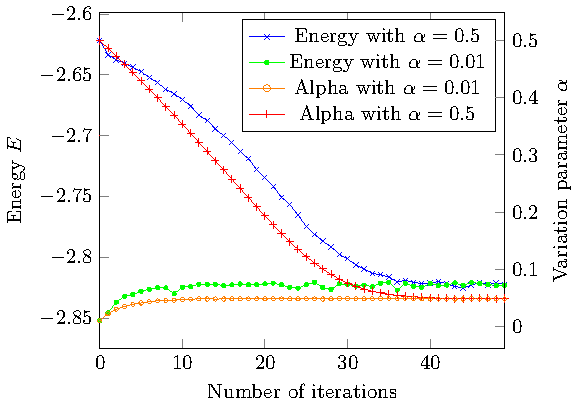
\includegraphics[scale=1 ]{graphs/he-e-alpha-iterations.pdf}
  \caption{
  	Calculated $E$ as a function of $\alpha$ using two different starting values for$\alpha_0$. Notice that $\alpha$ converges monotonically (increasing or decreasing) while this is not necessarily true for the energy due to the integration not being exact. Nonetheless, a very accurate result can be found: $E_{\alpha_0 = 0.5} =  $ and $E_{\alpha_0 = 0.5} =  $
  	%TODO: This was already mentioned in the text. I should only be in one place!
  	}
  \label{fig:He_it}
  \end{center}
\end{figure}
 
